\documentclass[]{elsarticle} %review=doublespace preprint=single 5p=2 column
%%% Begin My package additions %%%%%%%%%%%%%%%%%%%
\usepackage[hyphens]{url}

  \journal{An awesome journal} % Sets Journal name


\usepackage{lineno} % add
\providecommand{\tightlist}{%
  \setlength{\itemsep}{0pt}\setlength{\parskip}{0pt}}

\usepackage{graphicx}
\usepackage{booktabs} % book-quality tables
%%%%%%%%%%%%%%%% end my additions to header

\usepackage[T1]{fontenc}
\usepackage{lmodern}
\usepackage{amssymb,amsmath}
\usepackage{ifxetex,ifluatex}
\usepackage{fixltx2e} % provides \textsubscript
% use upquote if available, for straight quotes in verbatim environments
\IfFileExists{upquote.sty}{\usepackage{upquote}}{}
\ifnum 0\ifxetex 1\fi\ifluatex 1\fi=0 % if pdftex
  \usepackage[utf8]{inputenc}
\else % if luatex or xelatex
  \usepackage{fontspec}
  \ifxetex
    \usepackage{xltxtra,xunicode}
  \fi
  \defaultfontfeatures{Mapping=tex-text,Scale=MatchLowercase}
  \newcommand{\euro}{€}
\fi
% use microtype if available
\IfFileExists{microtype.sty}{\usepackage{microtype}}{}
\bibliographystyle{elsarticle-harv}
\ifxetex
  \usepackage[setpagesize=false, % page size defined by xetex
              unicode=false, % unicode breaks when used with xetex
              xetex]{hyperref}
\else
  \usepackage[unicode=true]{hyperref}
\fi
\hypersetup{breaklinks=true,
            bookmarks=true,
            pdfauthor={},
            pdftitle={Practical Applications for a Distributed Modeling Framework for Protected Data},
            colorlinks=false,
            urlcolor=blue,
            linkcolor=magenta,
            pdfborder={0 0 0}}
\urlstyle{same}  % don't use monospace font for urls

\setcounter{secnumdepth}{0}
% Pandoc toggle for numbering sections (defaults to be off)
\setcounter{secnumdepth}{0}

\newlength{\cslhangindent}
\setlength{\cslhangindent}{1.5em}
\newenvironment{cslreferences}%
  {\setlength{\parindent}{0pt}%
  \everypar{\setlength{\hangindent}{\cslhangindent}}\ignorespaces}%
  {\par}

% Pandoc header



\begin{document}
\begin{frontmatter}

  \title{Practical Applications for a Distributed Modeling Framework for
Protected Data}
    \author[Johns Hopkins Bloomberg School of Public Health]{John
Muschelli III\corref{Corresponding Author}}
   \ead{jmusche1@jhu.edu} 
      \address[Johns Hopkins Bloomberg School of Public
Health]{Department of Biostatistics, 615 N Wolfe St, Baltimore MD,
21205}
    
  \begin{abstract}
  We present 2 practical approaches to fitting generalized linear models
  in a distributed framework. The use case for this framework is where
  multiple sites (e.g.~hospitals) have data with protected or private
  information that cannot be shared, but aggregated data can be, and
  each site can send aggregated data across the internet.\\
  We present the first strategy: using synced folder services, such as
  Dropbox or Box Sync, to share the aggregated data. The second strategy
  involves creating an application programming interface (API), where
  sites submit the data to this service. This work relies on the R
  statistical software; we provide an R package of examples and code to
  create an API on DigitalOcean.
  \end{abstract}
  
 \end{frontmatter}

\hypertarget{introduction}{%
\section{Introduction}\label{introduction}}

We introduce a distrbuted framework to analyze data from multiple
sources with the data being properly siloed. The motivation for this
problem is simple: we would like to fit a generalized linear model (GLM)
on data from multiple sites (e.g.~hospitals), where the indvidual
patient-level data or otherwise private data never leaves the server
(siloed), which is usually behind a firewall. The idea is that a model
is specified, and sent to each site where a summary statistic is
computed and returned to the modeling service/site. The model is then
updated and, if necessary, the process is completed until the model is
fit until convergence. The goal is to fit the exact model as if the full
data was accessible.

The alternatives to this process is meta-analysis, one-step solutions,
or remote analysis servers {[}O'Keefe and Good (2008);{]}. There are
drawbacks to a meta-analysis approach in that the model and statistics
must be specified and commonly the data is gathered \textbf{once} from
each site. Also, if sites present estimates from models with different
predictors, it is unclear how meta-analysis adequately handles this
variability. The process below ensures that the same model, with the
same predictors, is fit at each site. Any updated analysis requires
additional correspondence between the modeler and the site data analyst,
which slows down the process of analysis and creates more hurdles.

The work presented here is almost identical to Grid Binary LOgistic
REgression (GLORE) (Wu et al., 2012), its Bayesian analog EXpectation
Propagation LOgistic REgRession (EXPLORER) (Wang et al., 2013), and
Secure Pooled Analysis acRoss K-sites (SPARK) (El Emam et al., 2013). A
few of the differences are: GLORE and EXPLORER focus primarily on only
logistic regression, SPARK works for all GLMs like the proposed method.
GLORE and SPARK are iterative requiring all sites to provide updates
until the next estimate can be achieved, like the current method;
EXPLORER is iterative but asynchronous so that sites can share updates
without coordination. SPARK additionally compute on encrypted data,
which allows for higher security; EXPLORER uses random matrix
implementations to increase security, but required inter-site
communication. Similarly, Wang et al. (2017) show an iterative method
for regularized/sparse model fitting. Jordan et al. (2019) present a
general framework by sending surrogate likelihood information in an
iterative way, which generalizes over GLMs, and they examples of
M-estimators, regularized/penalized models, and Bayesian models. All
previous solutions do not provide practical steps or tutorials to set up
a system, however.

To alleviate the need for iterative processes, one-shot solutions have
been presented. For example, One-shot Distributed Algorithm to perform
Logistic regressions (ODAL) (Duan et al., 2019) is a distributed
estimation procedure for a logistic model. for a given \(\beta\),
compute gradients of a likelihood and use these computed gradients to
inform the estimate of \(\beta\), but only with one iteration. They have
shown to get close estimates to the ``true model'', which would be the
model fit if all data was included. The work is expanded upon in
Robust-ODAL (Tong et al., 2020), where median gradients are estimated as
opposed to mean gradients, to diminish the influence of heterogeneous
site data. Other methods have shown that efficient one-step estimators
or averages perform well compared to an ``oracle model'' with the full
data (Battey et al., 2018; Zhang et al., 2013). These methods provide
great approximate solutions because 1) they are not iterative, 2) can be
computed in a privacy-preserving way, 3) can be robust to outlying data,
and 4) can be seen as likelihood updates. As a likelihood update, the
same process can be done with all but one site, determining the
robustness of the procedure in a sensitivity analysis. The downsides are
that the solution is approximate and if another model is to be run, the
whole process has to start again. Thus, we believe a remote analysis
server can be more general.

The work presented here is similar to that of O'Keefe and Good (2009) as
it has a remote analysis server, but with a main difference. Practical
implementations such as WebDISCO (web service for distributed Cox model
learning) exist, but these rely on a third-party service (at this time
the WebDISCO URL is a dead link) or a remote analysis server. In O'Keefe
and Good (2009) and most remote analysis servers, a full dataset
primarily exists. That is, the full data is available to that server,
but not those submitting the models. Moreover, these remote analysis
servers may be complicated and costly to set up. We will present a
system that does have the same constraints, as it will rely on a few
scripts or spooling up on a server on a low-cost online service with one
command.

That said, the previous methods and authors present solutions with a
series of additional checks with privacy-preserving measures which we
offload a bit on to the analyst at each separate site. We argue that
analysts already have this responsibility, but in a more informal way.
In some of the applications above, such as some of the one-shot
solutions, the model specification and updates are communicated by easy,
likely unsecure methods such as email. Thus, it would seem as though
iterative methods can give exact solutions in a secure way, but the
iterative process is burdensome. We wish to make the iterative process
easy and user-friendly.

We implemented a practical solution in an R package that allows
researchers to practically implement this system with real data. The
solution can be done a number of ways; we implemented 1) code to deploy
an API (application programming interface) on a remote server and 2)
scripts to calculate the model if using a synced folder, backed by
services such as Dropbox or Box Sync. This practical solution solves the
motivating problem, allowing us to fit many different types of models
with little technical overhead while keeping protected health
information (PHI) private.

\hypertarget{motivating-example}{%
\section{Motivating Example}\label{motivating-example}}

Let's estimate a GLM an outcome \(Y\) on a set of covariates \(X\), with
a link function \(G\). Let there be \(K\) hospitals, and \(Y\) and \(X\)
are on the data on all hospitals \(1, \dots, K\).

\[
g(E[Y | X]) = X\beta = \eta
\]

\[
u_i = \sum W (y_i - \mu) \frac{d\eta}{d\mu}x_i
\] where \[
W^{-1} = \left(\frac{d\eta}{d\mu}\right)^2V
\] and \(V\) is the variance function for the GLM evaluated at \(\mu\).

Let us also say that we are interested in \(p\) covariates, and
\(n_{k}\) is the total number of records at hospital \(k\) and
\(n = \sum_{1}^{k} n_{k}\), is the number of rows of \(Y\) and \(X\),
thus \(Y\) is an \(n\text{x}1\) vector and \(X\) is a \(n\text{x}p\)
matrix. To estimate \(\beta\), we would use: \[
(X'WX)^{-1} X'WY
\] where \(A = X'WX\) is a \(p\text{x}p\) matrix and \(X'Y\) is a
\(p\times{1}\) vector. But in our case, we can use \(u\), which is a
\(p\times 1\) vector

Since we don't have access to \(X\), but rather a series of \(X_{k}\),
\(k = 1, \dots, K\), we can use methods such as parallelized gradient
descent approaches (Mcdonald et al., 2009; Zinkevich et al., 2010) or
approximate maximum-likelihood approaches (Duncan, 1980). We choose to
use the Fisher scoring method outlined in McCulloch (2000) (page 42).
For generalized linear models, we simply need \(A}\) and \(u\)

Regardless, for almost any approach, the gradient or some
reduced-dimensional summary is required to be aggregated together to get
the estimate of \(\beta\) at the full population level. Now, if we
combine these models with models that require iterative fitting, such as
Generalized Linear Models (GLMs), there needs to be a lot of
communication and recomputation of summaries to get a final estimate.
These approaches work well in distributed computing systems (such as
computing clusters or GPUs), but have a much higher likelihood for
errors if human interaction is required at each iteration. This human
interaction is a common practice for most clinical data, which we wish
to show a simple solution to create the distributed computing much
simpler.

\hypertarget{methods}{%
\section{Methods}\label{methods}}

\texttt{plumber} is an R package that creates APIs (Application
programming interfaces) for and from R (Trestle Technology, LLC, 2018).
Though there are many frameworks to create APIs, such as Node.js and
Flask, we will focus on \texttt{plumber} for a number of reasons.
Overall, the API needs a computational backbone for this process to
work. As \texttt{plumber} is based in R, we know that the server will
have this already installed. Another reason is that the statisticians
and data analysts that will be running the models will likely be using a
statistical language, usually either R or Python. Though we will focus
on R, the ideas here can be extended to other languages and systems. We
are not experts in distributed computing, but would like to show how
this process is possible, overlooking obvious hurdles such as
authentication, load balancing, network issues, debugging, and overall
security on the server side.

The framework is as follows: a developer makes an R package with a
\texttt{plumber} API specification inside of it of the inputs and
outputs necessary for a specific model. For example, fitting a linear
model where the analyst specifies predictors and an outcome. The API has
endpoints that take in this model, run a specified computation on the
server (behind the hospital firewall), and returns a result that has
only aggregate data (such as a \(p\text{x}p\) matrix). The API logs the
output for potential future debugging and audits of the process. The
analysis system receives the output for each hospital, creates and
updated estimate of the model and runs the next iteration from each
hospital again until convergence. Thus, this system.

\begin{figure}
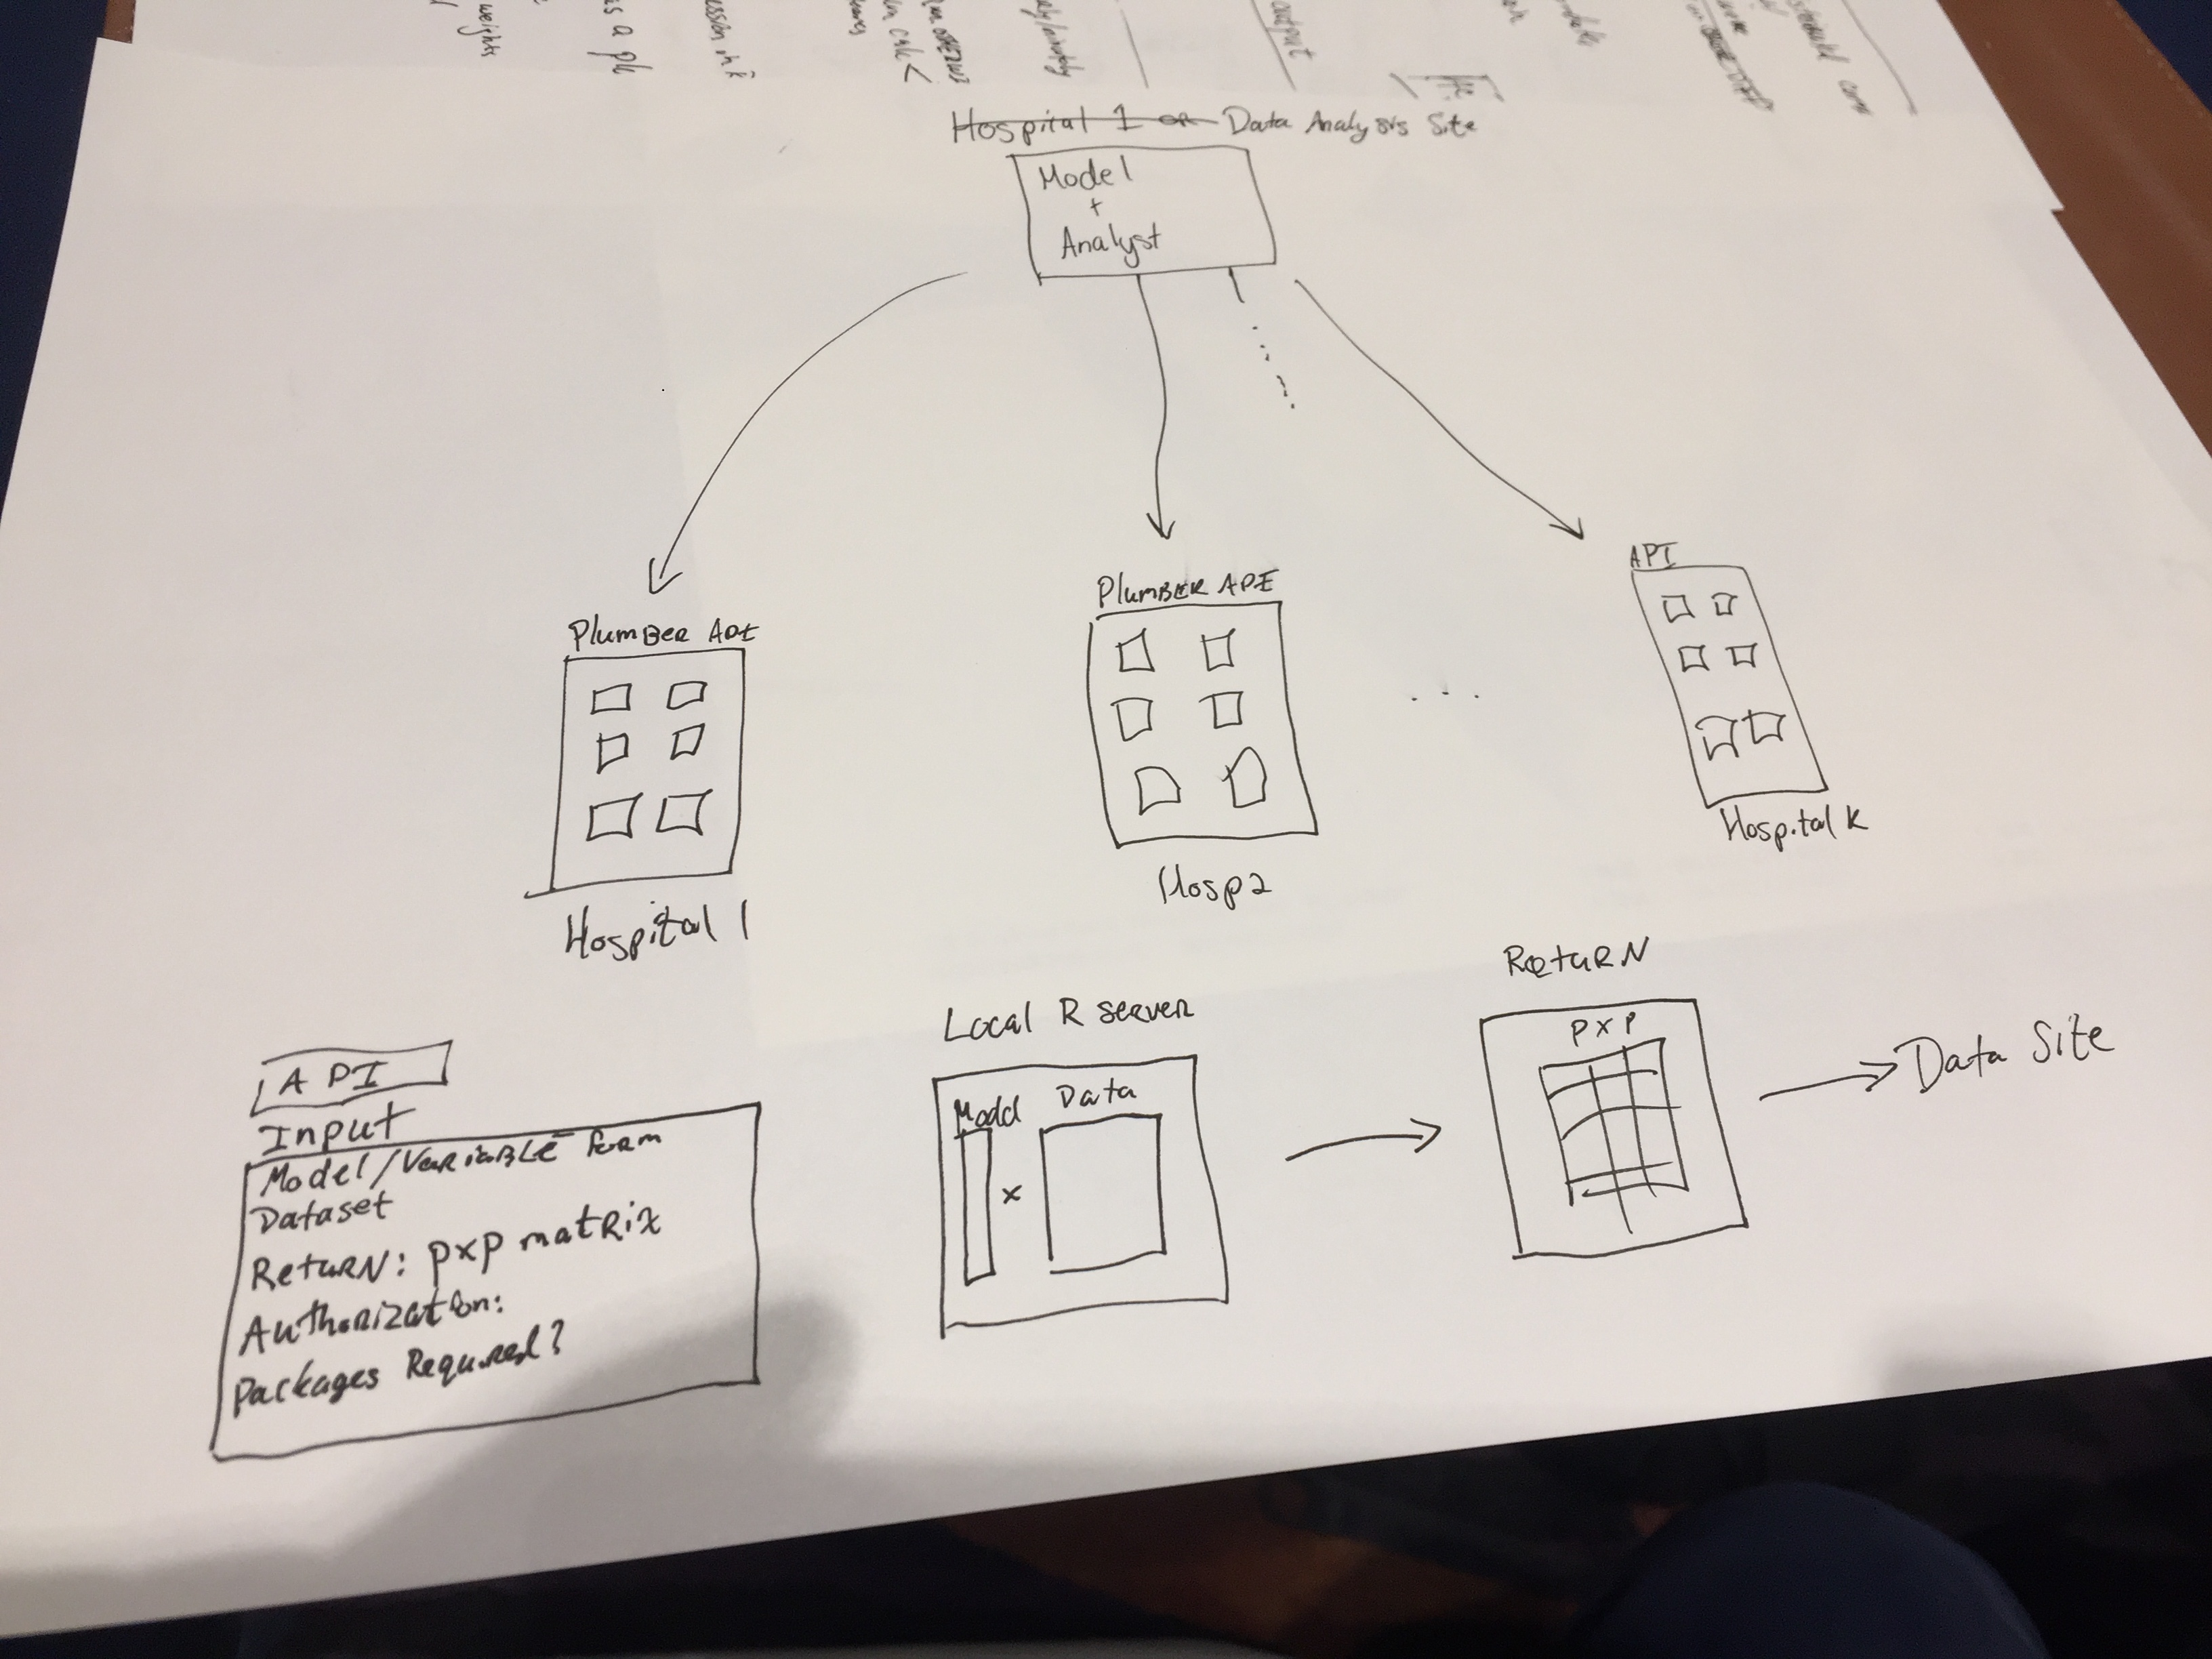
\includegraphics[width=1\linewidth]{sketch} \caption{Proposed Framework.  The modeler/analyst specifies a model, sends the model specification to an endpoint on each hospital API, a computation is run and returned to the analyst and aggregated (usually a gradient).  The model estimates are updated and the process repeats until the model converges.  }\label{fig:unnamed-chunk-1}
\end{figure}

\hypertarget{issues}{%
\section{Issues}\label{issues}}

Though the system may seem simple to describe, many obstacles exist.
Mainly opening any system that interacts with patient data or a database
(even if it were a spreadsheet) is a potential security risk which most
clinical centers will not allow. Though this caution is warranted, it
may be more secure than the alternative of sending estimates in other
communication systems such as email. Though emailing has the upside of a
human ensuring only aggregate data is transferred, it drastically
increases the potential for wrong computation. For example, the
\texttt{plumber} API can have checks on the data for missingness,
quality, the sample size is equal to that of the previous
iteration/model, and other issues, which may be done at varying levels
at each institution.

If the institution allows the API to be supported, then a server is
required, and usually an administrator to oversee it. This administrator
is usually trained in information systems or information technology,
which is likely not part of the clinical team. Thus, providing support
or interaction from the clinical team to the technical personnel can be
more costly than simply emailing estiamtes. Lastly, many institutions
and research groups would like a ``handle'' on what models are being fit
with their data, and thus limits on the API need to be created, which
may cause other issues or limitations on teh proposed framework.

These downsides are vastly outweighed when the API gets repeated use.
Thsu, fitting one model one time does not generally warrant the work
needed to set up this framework.

\hypertarget{references}{%
\section*{References}\label{references}}
\addcontentsline{toc}{section}{References}

\hypertarget{refs}{}
\begin{cslreferences}
\leavevmode\hypertarget{ref-battey2018distributed}{}%
Battey, H., Fan, J., Liu, H., Lu, J., Zhu, Z., 2018. Distributed testing
and estimation under sparse high dimensional models. Annals of
statistics 46, 1352.

\leavevmode\hypertarget{ref-duan2019odal}{}%
Duan, R., Boland, M.R., Moore, J.H., Chen, Y., 2019. ODAL: A one-shot
distributed algorithm to perform logistic regressions on electronic
health records data from multiple clinical sites., in: PSB. World
Scientific, pp. 30--41.

\leavevmode\hypertarget{ref-duncan1980approximate}{}%
Duncan, G.M., 1980. Approximate maximum likelihood estimation with data
sets that exceed computer limits. matrix 2, 1.

\leavevmode\hypertarget{ref-spark}{}%
El Emam, K., Samet, S., Arbuckle, L., Tamblyn, R., Earle, C.,
Kantarcioglu, M., 2013. A secure distributed logistic regression
protocol for the detection of rare adverse drug events. Journal of the
American Medical Informatics Association 20, 453--461.

\leavevmode\hypertarget{ref-jordan2019communication}{}%
Jordan, M.I., Lee, J.D., Yang, Y., 2019. Communication-efficient
distributed statistical inference. Journal of the American Statistical
Association 114, 668--681.

\leavevmode\hypertarget{ref-mcculloch2000generalized}{}%
McCulloch, C.E., 2000. Generalized linear models. Journal of the
American Statistical Association 95, 1320--1324.

\leavevmode\hypertarget{ref-mcdonald2009efficient}{}%
Mcdonald, R., Mohri, M., Silberman, N., Walker, D., Mann, G.S., 2009.
Efficient large-scale distributed training of conditional maximum
entropy models, in: Advances in Neural Information Processing Systems.
pp. 1231--1239.

\leavevmode\hypertarget{ref-o2008remote}{}%
O'Keefe, C.M., Good, N.M., 2008. A remote analysis server-what does
regression output look like?, in: International Conference on Privacy in
Statistical Databases. Springer, pp. 270--283.

\leavevmode\hypertarget{ref-o2009regression}{}%
O'Keefe, C.M., Good, N.M., 2009. Regression output from a remote
analysis server. Data \& Knowledge Engineering 68, 1175--1186.

\leavevmode\hypertarget{ref-tong2020robust}{}%
Tong, J., Duan, R., Li, R., Scheuemie, M.J., Moore, J.H., Chen, Y.,
2020. Robust-ODAL: Learning from heterogeneous health systems without
sharing patient-level data, in: Pacific Symposium on Biocomputing.
Pacific Symposium on Biocomputing. World Scientific, p. 695.

\leavevmode\hypertarget{ref-plumber}{}%
Trestle Technology, LLC, 2018. plumber: An API generator for R.

\leavevmode\hypertarget{ref-wang2017efficient}{}%
Wang, J., Kolar, M., Srebro, N., Zhang, T., 2017. Efficient distributed
learning with sparsity, in: Proceedings of the 34th International
Conference on Machine Learning-Volume 70. JMLR. org, pp. 3636--3645.

\leavevmode\hypertarget{ref-explorer}{}%
Wang, S., Jiang, X., Wu, Y., Cui, L., Cheng, S., Ohno-Machado, L., 2013.
EXpectation propagation LOgistic REgRession (EXPLORER): Distributed
privacy-preserving online model learning. Journal of biomedical
informatics 46, 480--496.

\leavevmode\hypertarget{ref-glore}{}%
Wu, Y., Jiang, X., Kim, J., Ohno-Machado, L., 2012. G rid binary LO
gistic RE gression (GLORE): Building shared models without sharing data.
Journal of the American Medical Informatics Association 19, 758--764.

\leavevmode\hypertarget{ref-zhang2013communication}{}%
Zhang, Y., Duchi, J.C., Wainwright, M.J., 2013. Communication-efficient
algorithms for statistical optimization. The Journal of Machine Learning
Research 14, 3321--3363.

\leavevmode\hypertarget{ref-zinkevich2010parallelized}{}%
Zinkevich, M., Weimer, M., Li, L., Smola, A.J., 2010. Parallelized
stochastic gradient descent, in: Advances in Neural Information
Processing Systems. pp. 2595--2603.
\end{cslreferences}


\end{document}

